\documentclass[10pt,spanish,aspectratio=1610]{beamer}
\usepackage[utf8]{inputenc}
\usepackage{amsmath}
\usepackage{graphicx}
\usepackage{amssymb}
\usepackage[spanish]{babel}
\spanishdecimal{.}
\usepackage{subfig}
\usepackage{fancyhdr}
\usepackage{pstricks}
\usepackage{verbatim}
\usepackage[ruled]{algorithm2e}
\usepackage[absolute, overlay]{textpos}
\usefonttheme{professionalfonts}
%\usepackage{ragged2e}
%\usepackage[natbibapa]{apacite}
% \bibliographystyle{apacite} % This is the style you should use with `apacite`.
%\justifying
\DeclareMathOperator{\atantwo}{atan2}
\newcommand\ddfrac[2]{\frac{\displaystyle #1}{\displaystyle #2}}
\usetheme{Boadilla}
\setbeamercovered{transparent}
\beamertemplatenavigationsymbolsempty
\setbeamertemplate{frametitle}
{
  \leavevmode
  \hbox{
  \begin{beamercolorbox}[wd=0.6\paperwidth,left]{frametitle}
    \usebeamerfont{frametitle}\insertframetitle
  \end{beamercolorbox}
  \begin{beamercolorbox}[wd=0.4\paperwidth,center]{frametitle}
    \usebeamerfont{frametitle}\hfill\small{\thesection. \insertsection}
  \end{beamercolorbox}
  }
}
\setbeamertemplate{footline}
{
  \leavevmode%
  \hbox{%
    \begin{beamercolorbox}[colsep=-0.5pt,wd=.33\paperwidth,ht=3ex,dp=1.5ex,center]{author in head/foot}%
      \usebeamerfont{author in head/foot}\insertshortauthor~~ (\insertshortinstitute)
    \end{beamercolorbox}%
    \begin{beamercolorbox}[colsep=-0.5pt,wd=.34\paperwidth,ht=3ex,dp=1.5ex,center]{date in head/foot}%
      \usebeamerfont{author in head/foot}\insertshorttitle
    \end{beamercolorbox}%
    \begin{beamercolorbox}[colsep=-0.5pt,wd=.33\paperwidth,ht=3ex,dp=1.5ex,right]{author in head/foot}%
      \usebeamerfont{author in head/foot}\insertshortdate{}\hspace*{2em}\scriptsize{\insertframenumber{}}\hspace*{1ex}
    \end{beamercolorbox}
  }
}

\begin{document}
\renewcommand{\tablename}{Tabla}
\renewcommand{\figurename}{Figura}

\title[Robocup@Home Beginners]{Curso Introductorio para la Categoría\\Robocup@Home Beginners}
\author[Marco Negrete y Luis González]{Instructores: \\ Marco Antonio Negrete Villanueva \\ Luis González Nava}
\institute[FI, UNAM]{Facultad de Ingeniería, UNAM}
\date[EIR 2020]{Escuela de Invierno de Robótica 2020, Saltillo, México.}

\begin{frame}
\titlepage
\end{frame}

\begin{frame}\frametitle{Objetivos}
  \begin{itemize}
  \item Revisar el hardware necesario para tener un robot de servicio doméstico: sensores y actuadores necesarios.
  \item Dar un panorama general del software necesario para desarrollar un robot de servicio doméstico.
  \item Revisar las herramientas disponibles para cubrir las habilidades requeridas en la categoría @Home Beginners:
    \begin{itemize}
    \item Navigation stack (planeación de movimientos)
    \item Pocketsphinx (reconocimiento de voz)
    \item Sound Play (para síntesis de voz)
    \item OpenCV (reconocimiento de objetos y rostros)
    %\item MoveIt (para manipulación de objetos)
    \end{itemize}
  \end{itemize}
\end{frame}

%%%%%%%%%%
%%%%%%%%%% ANTECEDENTES
%%%%%%%%%%
\section{Antecedentes}
\begin{frame}\frametitle{La categoria @Home}
  \begin{columns}
    \begin{column}{0.5\textwidth}
      Su objetivo es el desarrollo de robots de servicio doméstico y está enfocada principalmente en las siguientes áreas:
      \begin{itemize}
      \item Interacción humano-robot
      \item Navegación en ambientes dinámicos
      \item Visión computacional y reconocimiento de objetos
      \item Manipulación de objetos
      \item Comportamientos adaptables
      \item Integración de Comportamientos
      \item Estandarización e integración de sistemas
      \end{itemize}
    \end{column}
    \begin{column}{0.4\textwidth}
      \centering
      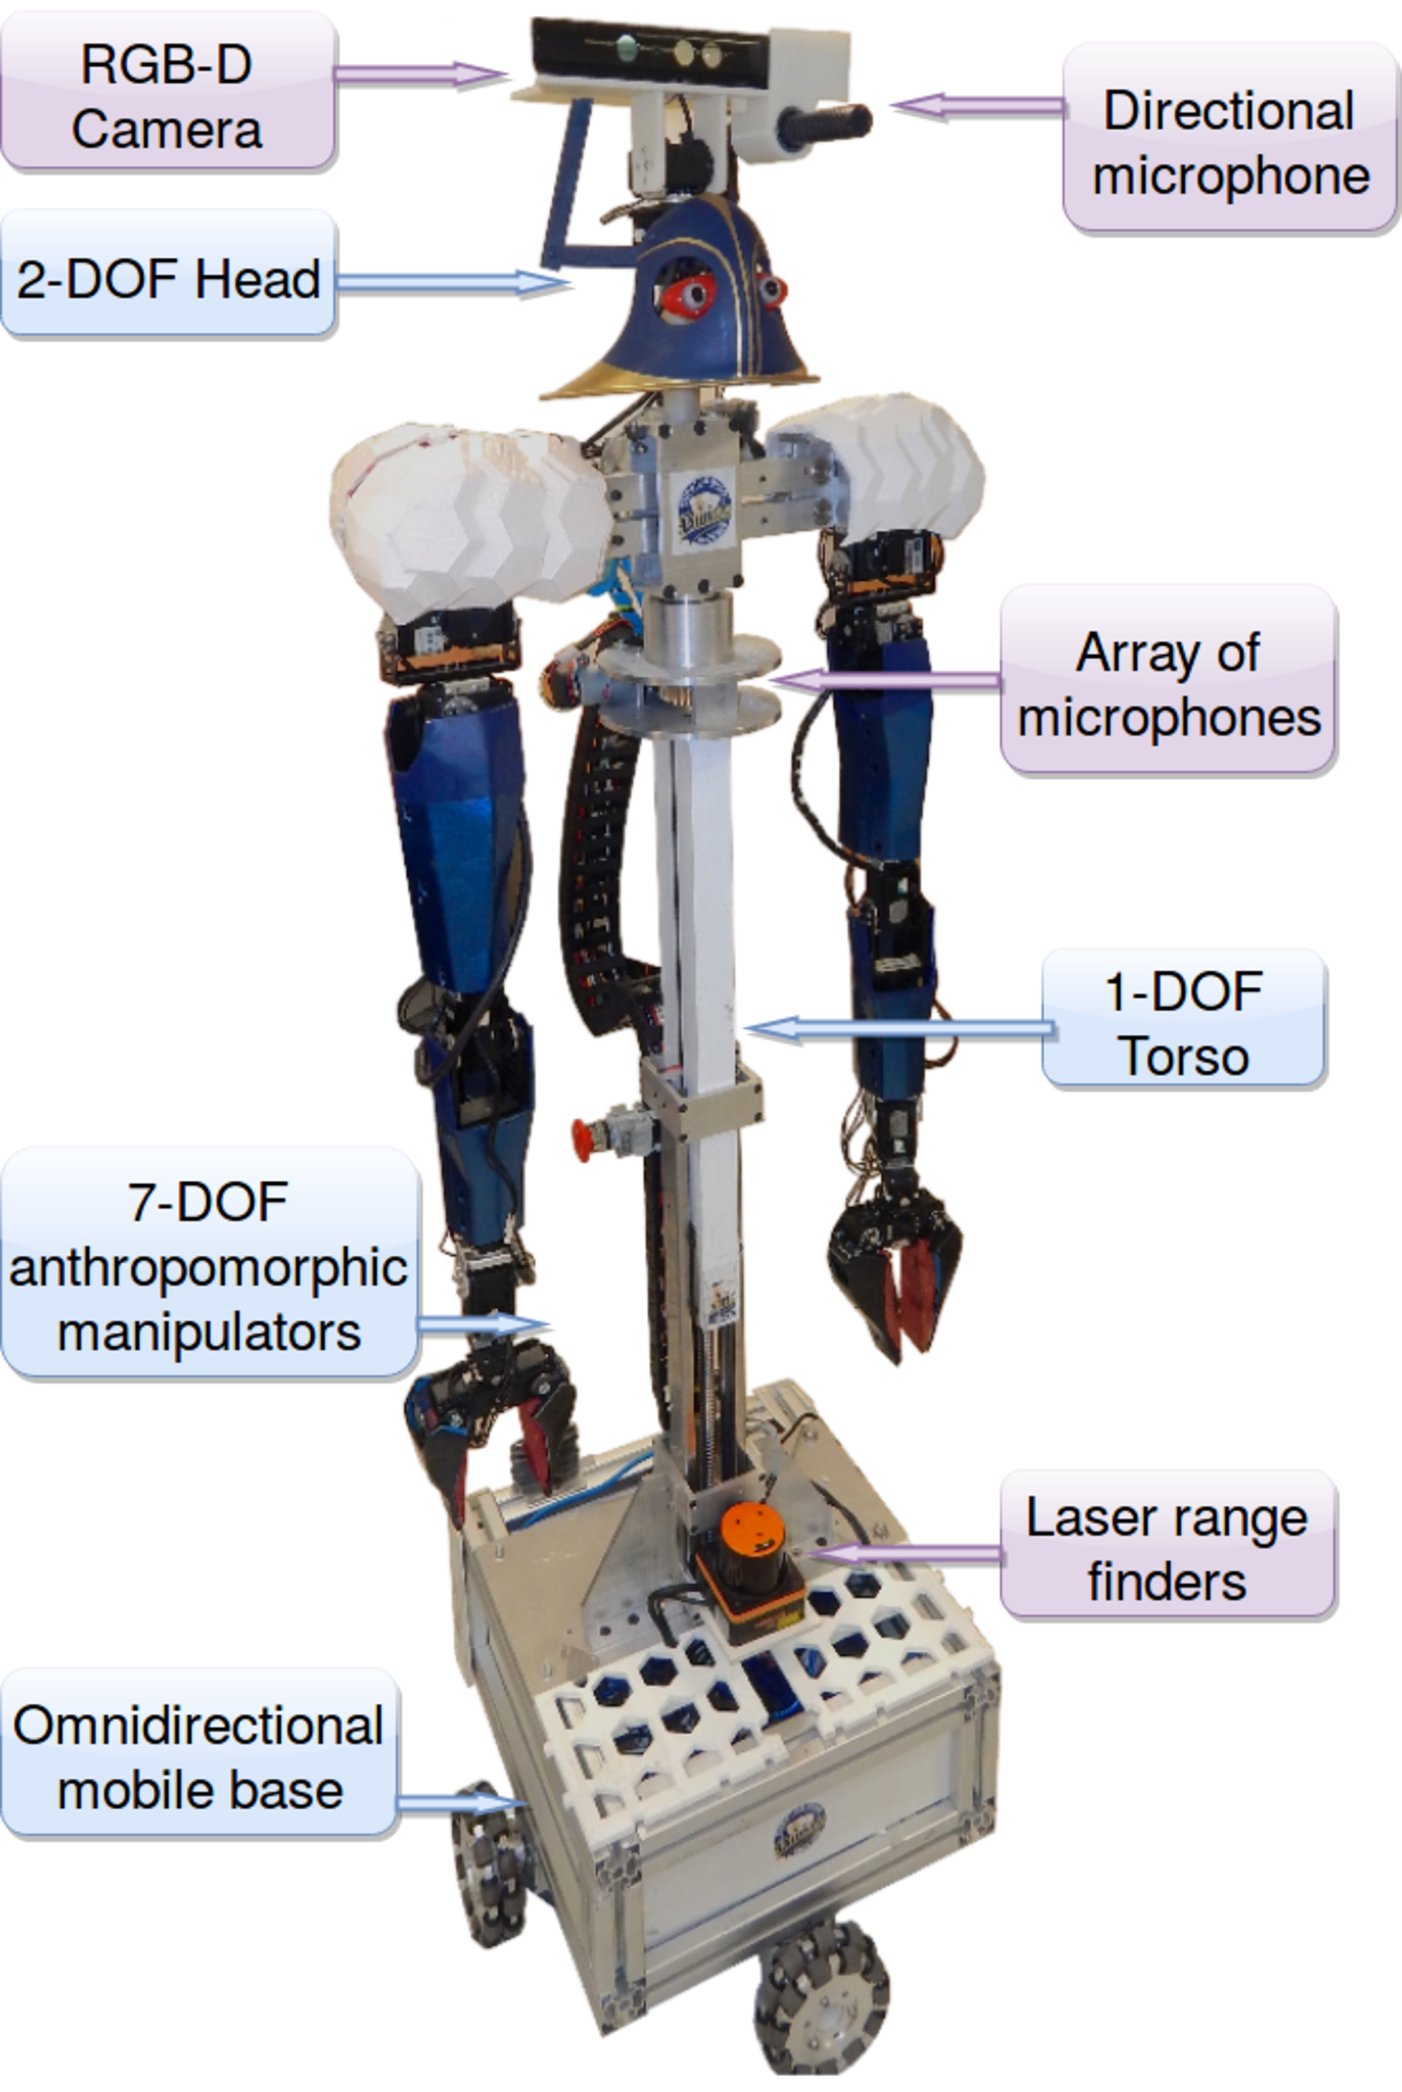
\includegraphics[width=0.9\textwidth]{Figures/Justina.pdf}
    \end{column}
  \end{columns}
\end{frame}

\begin{frame}\frametitle{La categoria @Home Beginners}
  \begin{figure}
    \centering
    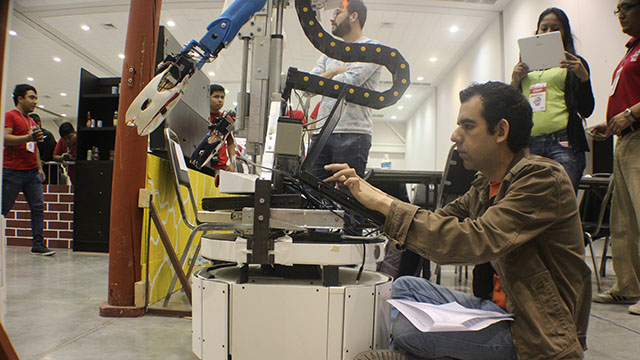
\includegraphics[width=0.5\textwidth]{Figures/AtHomeBeginners.jpg}
  \end{figure}

  Esta competencia presenta un desafío introductorio a la categoría de @Home Major, basándose en una etapa de pruebas y una final.
      \begin{itemize}
      \item En la etapa de pruebas se evalúan funcionalidades básicas por separado:
        \begin{itemize}
        \item Navegación
        \item Reconocimiento de objetos
        \item Manipulación
        \item Reconocimiento de voz
        \end{itemize}
      \item La prueba final es una integración de las habilidades anteriores.
      \item El robot debe ejecutar un comando del tipo ``Bring [OBJETO] from [LUGAR]''.
      \end{itemize}
\end{frame}

\begin{frame}\frametitle{Hardware necesario: Base móvil}
  \begin{columns}
    \begin{column}{0.5\textwidth}
      \begin{itemize}
      \item De preferencia, debe ser omnidireccional
      \item Turtle Bot (\url{https://www.turtlebot.com/})
      \item Festo Robotino (\url{https://wiki.openrobotino.org/})
      \item DIY: 3 ó 4 motores de corriente directa con ruedas omnidireccionales, 2 tarjetas Roboclaw, baterías de LiPo y chasis de alumnio estructural.
      \end{itemize}
    \end{column}
    \begin{column}{0.5\textwidth}
      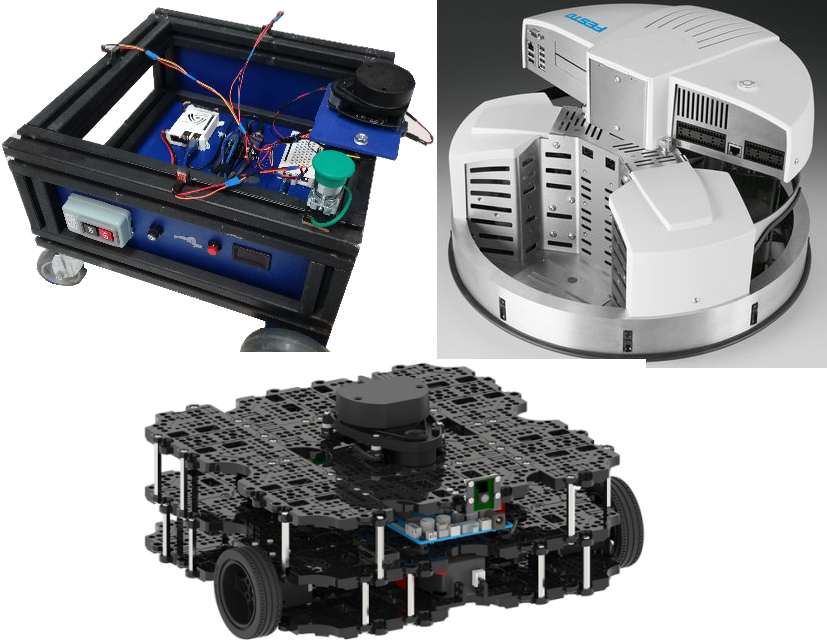
\includegraphics[width=\textwidth]{Figures/Bases.png}
    \end{column}
  \end{columns}
\end{frame}

\begin{frame}\frametitle{Hardware necesario: Cámaras}
  \begin{columns}
    \begin{column}{0.45\textwidth}
      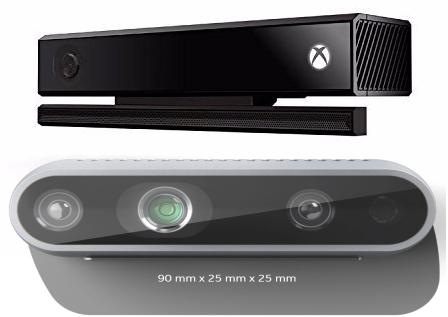
\includegraphics[width=\textwidth]{Figures/Cameras.jpg}
    \end{column}
    \begin{column}{0.5\textwidth}
      \begin{itemize}
      \item Se pueden usar sólo cámaras RGB, pero es altamente recomendable tener información de profundidad.
      \item Kinect (\url{https://github.com/OpenKinect/libfreenect2})
      \item Intel RealSense (\url{https://github.com/IntelRealSense/librealsense})
      \item También se pueden usar cámaras estéreo, pero es mucho más sencillo usar cámaras con luz estructurada.
      \end{itemize}
    \end{column}
  \end{columns}
\end{frame}

\begin{frame}\frametitle{Hardware necesario: Sensor láser}
  \begin{columns}
    \begin{column}{0.5\textwidth}
      \begin{itemize}
      \item Hokuyo (\url{https://www.hokuyo-aut.jp/})
      \item RPLidar (\url{https://www.robotshop.com/en/slamtec.html})
      \item SICK (\url{https://www.sick.com/ag/en/detection-and-ranging-solutions/2d-lidar-sensors/c/g91900})
      \item El paquete \url{http://wiki.ros.org/urg_node} facilita su operación.
      \item Si no se tiene uno, se puede simular a partir de una cámara RGB-D con el paquete \url{http://wiki.ros.org/pointcloud_to_laserscan}.
      \end{itemize}
    \end{column}
    \begin{column}{0.4\textwidth}
      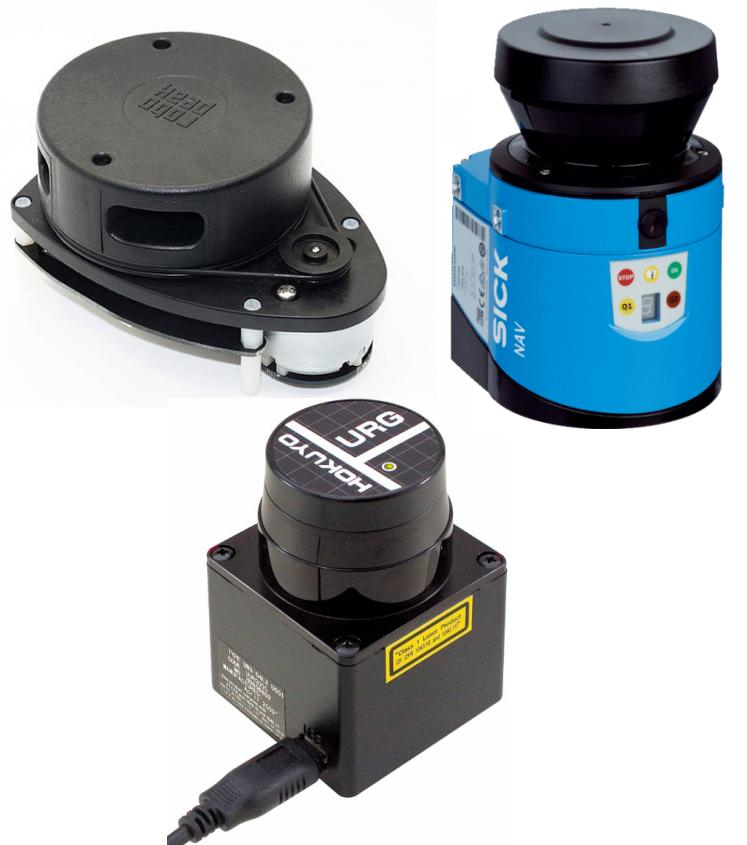
\includegraphics[width=\textwidth]{Figures/lasers.jpg}
    \end{column}
  \end{columns}
\end{frame}

\begin{frame}\frametitle{Hardware necesario: Manipulador}
  \begin{columns}
    \begin{column}{0.4\textwidth}
      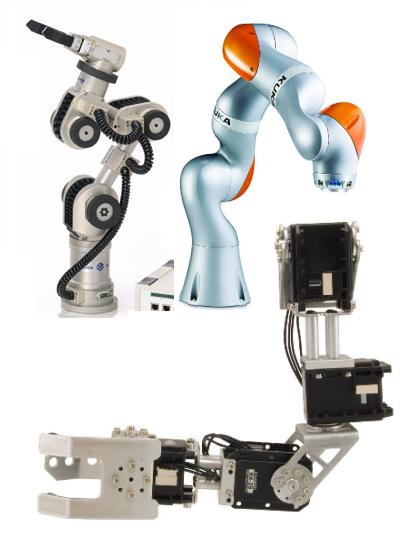
\includegraphics[width=\textwidth]{Figures/arms.jpg}
    \end{column}
    \begin{column}{0.5\textwidth}
      \begin{itemize}
      \item Son recomendables por lo menos 5 DOF.
      \item Kuka LBR iiwa (\url{http://wiki.ros.org/kuka})
      \item Neuronics Katana (\url{http://wiki.ros.org/katana})
      \item DIY: Servomotores y Brackets Dynamixel (\url{http://wiki.ros.org/dynamixel})
      \end{itemize}
    \end{column}
  \end{columns}
\end{frame}


\begin{frame}\frametitle{Configuraciones mínimas}
  \begin{itemize}
  \item Se requiere de un marco de referencia absoluto, comúnmente llamado \texttt{map}. En Rviz, \texttt{map} se selecciona como referencia global.
  \item La base móvil debe publicar su odometría y aceptar comandos de movimiento.
    \begin{itemize}
    \item Para la odometría, debe publicar la transformación de \texttt{odom} a \texttt{base\_link}.
    \item Para los comandos de movimiento, debe suscribirse al tópico \texttt{/cmd\_vel} de tipo \texttt{geometry\_msgs/Twist}.
    \end{itemize}
  \item Se requiere de un nodo que publique la transformación de \texttt{odom} a \texttt{map}.
    \begin{itemize}
    \item Si se está construyendo un mapa, esta transformación la publican paquetes como \texttt{gmapping} o \texttt{hector-mapping}.
    \item Si ya se tiene un mapa, la trasnformación la publica el nodo de localización, generalmente \texttt{amcl}. 
    \end{itemize}
  \item Se requiere de un archivo que describa la cinemática del robot (archivo \texttt{urdf}), es decir, el árbol de transformaciones. Se recomienda que el \textit{frame} raíz tenga el nombre \texttt{base\_link}. Ejemplo: \texttt{catkin\_ws/src/hardware/robot\_description/robotino.urdf}
    \item Cada \texttt{joint} del robot corresponderá a una transformación publicada por el nodo \texttt{robot\_state\_publisher}.
    \end{itemize}
\end{frame}

\begin{frame}\frametitle{Ejercicio}
  Ejecutar el comando \texttt{roslaunch bring\_up robotino\_simul.launch}. Debe aparecer un rviz como el siguiente:
  \begin{figure}
    \centering
    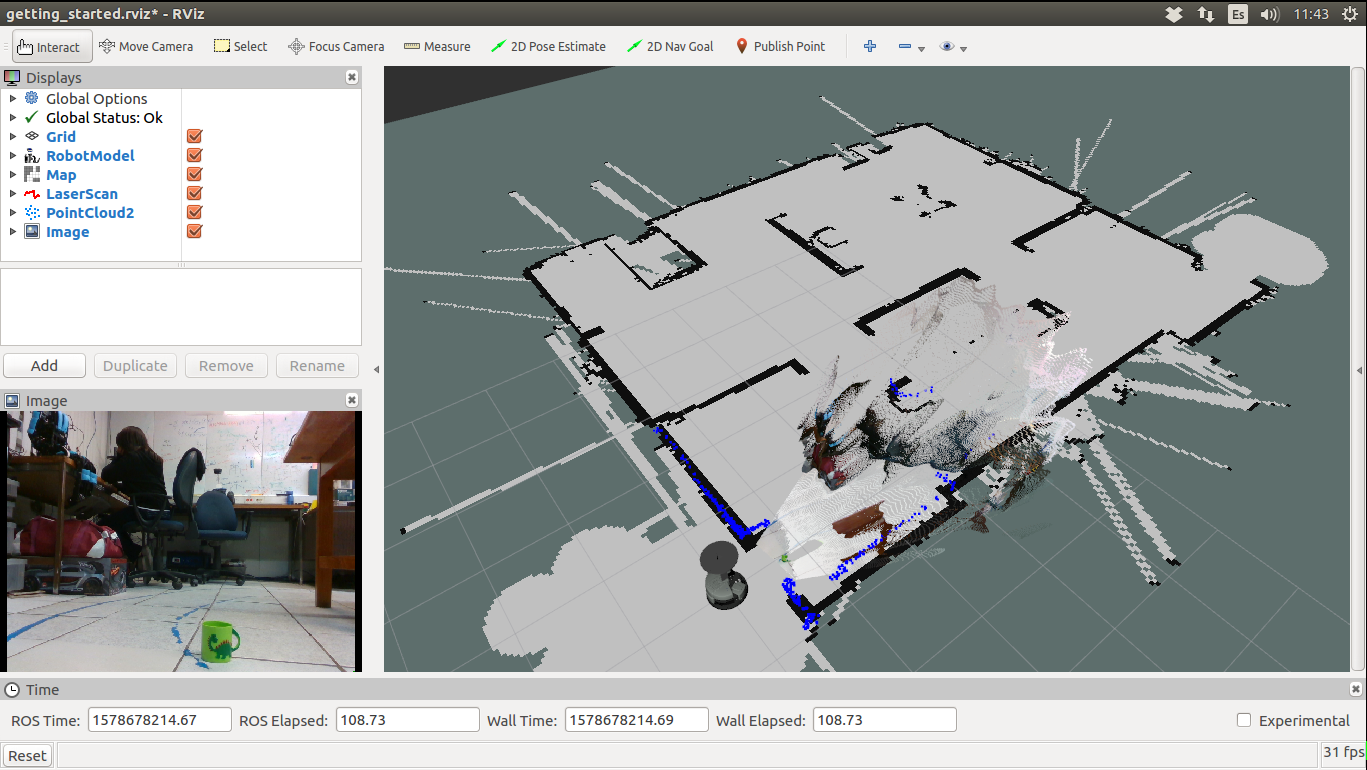
\includegraphics[width=0.7\textwidth]{Figures/RepoExample.png}
  \end{figure}
\end{frame}

\begin{frame}\frametitle{Ejercicio}
  \begin{enumerate}
  \item Ejecutar el comando \texttt{rosrun tf view\_frames} y verificar en el archivo resultante (\textit{frames.pdf}) las transformaciones y qué nodos las publican.
  \item Mediante el comando \texttt{rostopic info}, desplegar la información de los tópicos \texttt{/cmd\_vel} , \texttt{/scan} y \texttt{/camera/depth\_registered/points}.
  \item Detener la ejecución y modificar el archivo \texttt{catkin\_ws/src/bring\_up/launch/robotino\_simul.launch} para cambiar lo siguiente:
  \begin{itemize}
  \item La descripción del robot (\texttt{robotino.urdf} o \texttt{justina\_simple.urdf})
  \item El mapa del ambiente (Universum, Biorobotica o TMR\_2019)
  \end{itemize}
  \item Modificar el archivo \texttt{catkin\_ws/src/hardware/robot\_description/robotino.urdf} y ver qué sucede cuando:
  \begin{itemize}
  \item Se cambian los valores de la etiqueta \texttt{origin} en la línea 114.
  \item Se elimina alguno de los campos \texttt{<joint>}.
  \end{itemize}
\end{enumerate}
\end{frame}

%%%%%%%%%%
%%%%%%%%%% NAVEGACIÓN
%%%%%%%%%%
\section{Navegación}
\begin{frame}\frametitle{Navegación}
  \begin{textblock*}{0.4\textwidth}(15pt,55pt)
    \textbf{ Planeación de rutas. }\\Encontrar un mapeo: 
    \[P(\alpha): [0,1] \rightarrow Q_{free}\]
  \end{textblock*}
  \begin{textblock*}{0.35\textwidth}(310pt,27pt)
    \textbf{Mapeo: }Construir una representación del espacio:
    \[Q = Q_{free} \cup Q_{occupied}\]
  \end{textblock*}
  \begin{textblock*}{0.35\textwidth}(35pt,230pt)
    \textbf{Localización: }Determinar la configuración $q\in Q$ del robot.
  \end{textblock*}
  \begin{textblock*}{0.25\textwidth}(340pt,195pt)
    \textbf{Cobertura: }Mover al robot por todos los puntos $q\in Q_{free}$
  \end{textblock*}
  \centering  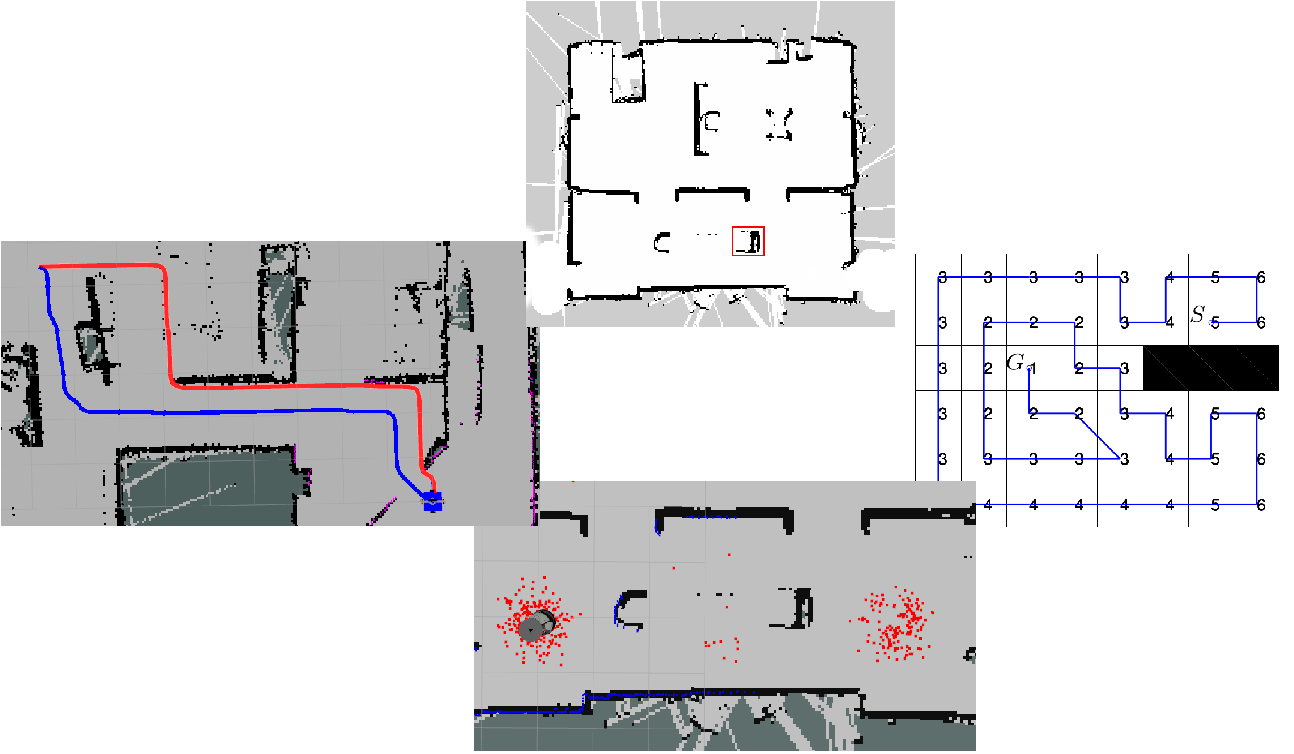
\includegraphics[width=0.9\textwidth]{Figures/MotionPlanningProblems.pdf}
\end{frame}

\begin{frame}\frametitle{Métodos de planeación de rutas}
  \begin{textblock*}{0.4\textwidth}(10pt,80pt)
    \textbf{ Métodos variacionales }\\Ejemplo:\\ Suavizado de una ruta
  \end{textblock*}
  \begin{textblock*}{0.35\textwidth}(305pt,27pt)
    \textbf{Búsqueda en grafos }\\Ejemplos: \\Dijkstra y A*
  \end{textblock*}
  \begin{textblock*}{0.3\textwidth}(50pt,235pt)
    \textbf{Basados en muestreo }\\Ejemplo: Rapidly Exploring Random Trees (RRT)
  \end{textblock*}
  \begin{textblock*}{0.25\textwidth}(355pt,195pt)
    \textbf{Geométricos }\\Ejemplo: \\ Grafo de visibilidad
  \end{textblock*}
  \centering
  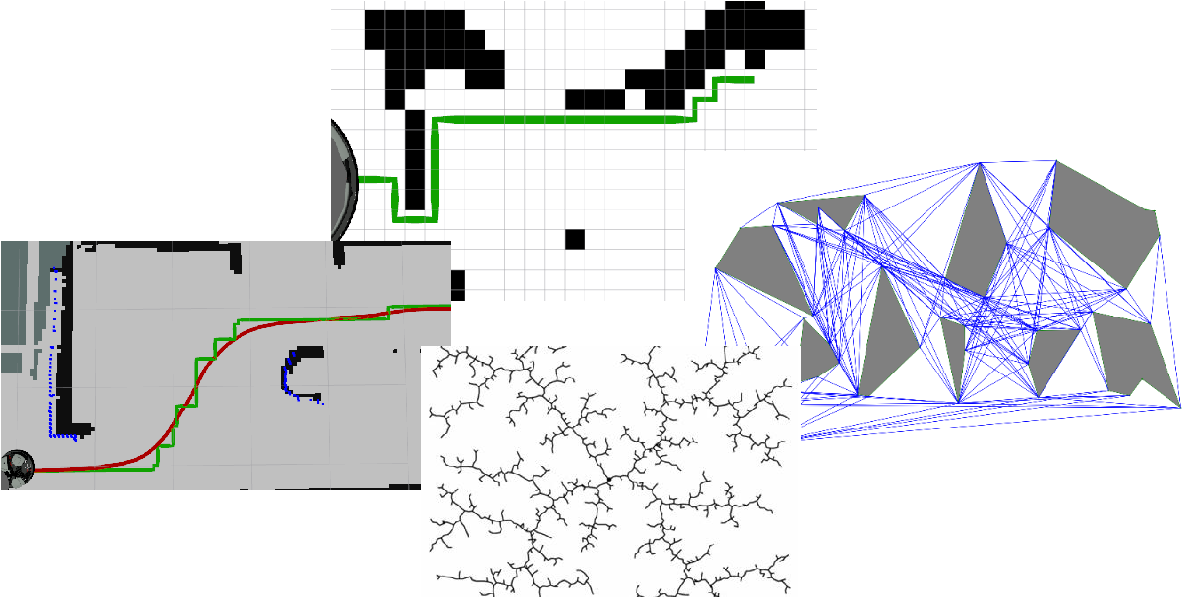
\includegraphics[width=0.95\textwidth]{Figures/PathPlanningMethods.pdf}
\end{frame}


\begin{frame}\frametitle{Métodos de localización y mapeo}
  \begin{columns}
    \begin{column}{0.45\textwidth}
      \textbf{Filtro de Kalman:} 
      \begin{itemize}
      \item Con base en un modelo, filtra el ruido de las mediciones de posición.
      \item Supone que la posición tiene una distribución unimodal (normal).
      \item Converge sólo si la estimación inicial está cerca de la real.
      \item El número de estados crece con el número de marcas.
      \item Bajo costo computacional.
      \end{itemize}
      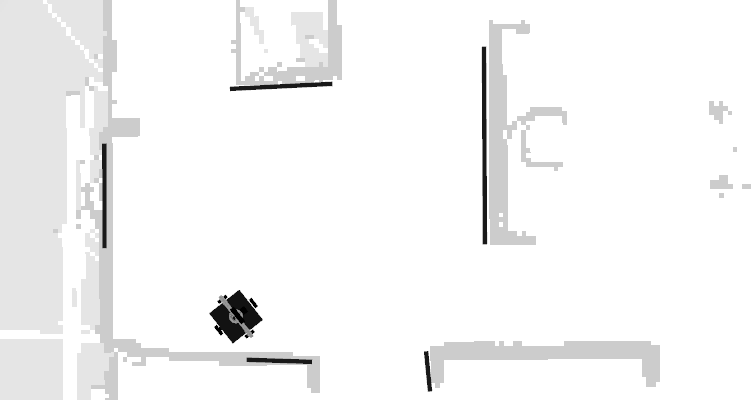
\includegraphics[width=0.95\textwidth]{Figures/LineExtractionLines.png}
    \end{column}
    \begin{column}{0.45\textwidth}
      \textbf{Filtro de Partículas:}
      \begin{itemize}
      \item También requiere de un modelo de movimiento.
      \item La distribución de probabilidad de la posición es multimodal.
      \item Funciona para cualquier estimación inicial de la posición.
        \item Cada partícula mantiene una estimación
      \item Alto costo computacional.
      \end{itemize}
      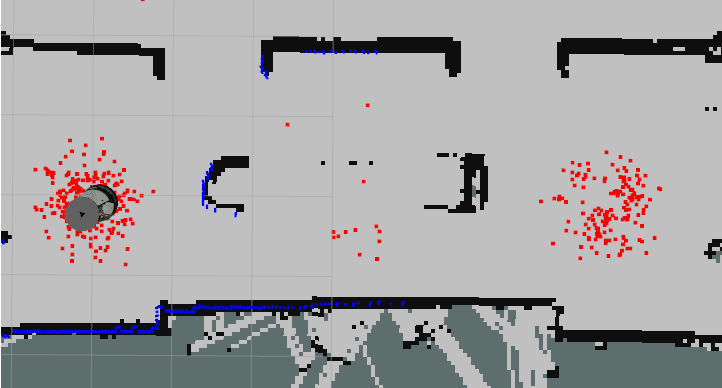
\includegraphics[width=0.95\textwidth]{Figures/ParticleFilter.png}
    \end{column}
  \end{columns}
\end{frame}


\begin{frame}\frametitle{El \textit{Navigation Stack} de ROS}
  Contiene varios paquetes para planeación de rutas, mapeo, localización y evasión de obstáculos (\url{http://wiki.ros.org/navigation}). Para este curso se usaron los siguientes:
  \begin{itemize}
  \item \texttt{map\_server}: Lee el mapa de dos archivos, una imagen \texttt{.pgm} y un \texttt{yaml} con meta datos. Publica el mapa usando un mensaje de tipo \texttt{nav\_msgs/OccupancyGrid}.
  \item \texttt{amcl}: Realiza la localización usando el mapa, la odometría y las lecturas del láser. Publica la transformación de \texttt{odom} a \texttt{map}.
    \texttt{move\_base}: Realiza la mayor parte de las tareas de planeación de movimientos, para lo que usa los paquetes:
    \begin{itemize}
    \item \texttt{dwa\_local\_planner}
    \item \texttt{navfn}
    \item \texttt{costmap\_2d}
    \end{itemize}
  \end{itemize}
\end{frame}

\begin{frame}\frametitle{Ejercicio}
  \begin{enumerate}
  \item Ejecutar los comandos
    \begin{itemize}
    \item \texttt{roslaunch bring\_up robotino\_simul.launch}
    \item \texttt{roslaunch bring\_up navigation\_move\_base.launch}
    \end{itemize}
  \item En el cuadro \textit{Displays} de \textit{Rviz} agregar los tópicos:
    \begin{itemize}
    \item \texttt{/move\_base/DWAPlannerROS/global\_plan}
    \item \texttt{/move\_base/DWAPlannerROS/local\_plan}
    \item \texttt{/move\_base/global\_costmap/costmap}
    \end{itemize}
    \item Fijar una meta con el botón \textit{2D Nav Goal} y observar el comportamiento.
  \end{enumerate}
\end{frame}

\begin{frame}\frametitle{Ejercicio}
  \begin{enumerate}
  \item Detener la ejecución de \texttt{navigation\_move\_base.launch}.
  \item En el archivo \texttt{catkin\_ws/src/config\_files/move\_base\_params/costmap\_common\_params.yaml}:
    \begin{itemize}
    \item Cambiar \texttt{cost\_scaling\_factor} a 1.0
    \item Cambiar \texttt{inflation\_radius} a 2.5
    \end{itemize}
  \item Relanzar \texttt{navigation\_move\_base.launch} y observar qué sucede.
  \item Detener la ejecución de \texttt{navigation\_move\_base.launch}.
  \item En el archivo \texttt{catkin\_ws/src/config\_files/move\_base\_params/dwa\_local\_planner\_params.yaml}:
    \begin{itemize}
    \item Cambiar \texttt{max\_vel\_x} a 2.0
    \item Cambiar \texttt{max\_trans\_vel} a 2.0
    \item Cambiar \texttt{acc\_lim\_x} a 2.0
    \end{itemize}
  \item Relanzar \texttt{navigation\_move\_base.launch} y observar qué sucede.
  \end{enumerate}
  \textbf{Nota:} En un robot real, los parámetros anteriores deben ser ligeramente menores a las capacidades físicas de la base móvil. 
\end{frame}

%%%%%%%%%%
%%%%%%%%%% RECONOCIMIENTO DE VOZ
%%%%%%%%%%
\section{Reconocimiento de voz}
\begin{frame}\frametitle{Reconocimiento de voz con Pocketsphinx}
  Pocketsphinx es un \textit{toolkit} open source desarrollado por la Universidad de Carnegie Mellon (\url{https://cmusphinx.github.io/}).
  \begin{itemize}
  \item Aunque el toolbox original no está hecho específicamente para ROS, ya existen varios repositorios con nodos ya implementados que integran ROS y Pocketsphinx:
    \begin{itemize}
    \item \url{https://github.com/mikeferguson/pocketsphinx}
    \item \url{https://github.com/Pankaj-Baranwal/pocketsphinx}
    \end{itemize}
  \item El usuario debe estar agregado al grupo \textit{audio} para el correcto funcionamiento: \texttt{sudo usermod -a -G audio <user\_name>}
  \end{itemize}
  \begin{itemize}
  \item Se puede hacer reconocimiento usando una lista de palabras, un modelo de lenguaje o una gramática.
  \item Se utilizarán gramáticas y sus correspondientes diccionarios.
  \item Para construir diccionarios, visitar \url{https://cmusphinx.github.io/wiki/tutorialdict/}
  \item Para construir gramáticas, visitar \url{https://www.w3.org/TR/2000/NOTE-jsgf-20000605/}
  \end{itemize}
\end{frame}

\begin{frame}\frametitle{Ejercicio}
  \begin{enumerate}
  \item Ejecutar el comando \texttt{roslaunch bring\_up pocketsphinx\_test.launch}
  \item Verificar los volúmenes del micrófono
  \item Revisar el archivo \texttt{catkin\_ws/src/pocketsphinx/vocab/voice\_cmd.gram} para ver las frases que se pueden reconocer de acuerdo con la gramática.
  \item Probar el reconocimiento de voz.
  \item Detener la ejecución. En el archivo \texttt{catkin\_ws/src/bring\_up/launch/pocketsphinx\_text.launch}:
    \begin{enumerate}
    \item Cambiar el valor del parámetro \texttt{gram} de \texttt{.../voice\_cmd} a \texttt{.../restaurant}
    \item Cambiar el valor del parámetro \texttt{dict} de \texttt{../voice\_cmd.dic} a \texttt{restaurant.dict}
    \item Cambiar el valor de \texttt{grammar} de \texttt{voice\_cmd} a \texttt{restaurant}
    \item Cambiar el valor de \texttt{rule} de \texttt{move2} a \texttt{command}
    \end{enumerate}
  \item Relanzar el archivo \texttt{pocketsphinx\_test.launch} y verificar el reconocimiento de acuerdo con la gramática del archivo \texttt{restaurant.gram}
  \end{enumerate}
\end{frame}

%%%%%%%%%%
%%%%%%%%%% SINTESIS DE VOZ
%%%%%%%%%%
\section{Síntesis de voz}
\begin{frame}\frametitle{Síntesis de voz con SoundPlay}
  \begin{itemize}
  \item Es un paquete que permite reproducir archivos \texttt{.wav} o \texttt{.ogg}, sonidos predeterminados y síntesis de voz.
  \item La síntesis de voz se hace utilizando Festival (\url{http://www.cstr.ed.ac.uk/projects/festival/}).
  \item Para sintetizar voz, basta con correr el nodo \texttt{soundplay\_node} y publicar un mensaje de tipo \texttt{sound\_play/SoundRequest} con lo siguiente:
    \begin{itemize}
    \item msg\_speech.sound   = -3                 
    \item msg\_speech.command = 1                  
    \item msg\_speech.volume  = 1.0                
    \item msg\_speech.arg2    = ``voz a utilizar''
    \item msg\_speech.arg = ``texto a sintetizar''
    \end{itemize}
  \end{itemize}
\end{frame}

\begin{frame}\frametitle{Ejercicio}
  \begin{enumerate}
  \item Ejecutar el comando \texttt{roslaunch bring\_up speech\_test.launch}
  \item Ejecutar el comando \texttt{rosrun speech\_syn speech\_test.py ``my first synthetized voice''}
  \end{enumerate}
\end{frame}

\begin{frame}\frametitle{Instalación de más voces}
  \begin{itemize}
  \item Las voces se pueden instalar con \texttt{sudo apt-get install festvox-<voz deseada>}
  \item Para ver qué voces se tienen instaladas: \texttt{ls /usr/share/festival/voices/english/}
  \end{itemize}
\end{frame}

\begin{frame}\frametitle{Ejercicio}
  \begin{enumerate}
  \item Instalar alguna voz.
  \item Verificar el nombre de la voz en el directorio \texttt{ls /usr/share/festival/voices/english/}
  \item Modificar el archivo \texttt{catkin\_ws/src/speech\_syn/scripts/speech\_test.py} y cambiar la voz a utilizar en el mensaje SoundRequest.
  \item El nombre de la voz se compone de \texttt{voice\_} más el nombre que aparece en la carpeta \texttt{voices/english}. 
  \end{enumerate}
\end{frame}

%%%%%%%%%%
%%%%%%%%%% VISIÓN
%%%%%%%%%%
\section{Visión}
\begin{frame}\frametitle{La biblioteca OpenCV}
  \begin{itemize}
  \item OpenCV es un conjunto de bibliotecas que facilita la implementación de algoritmos de visión computacional.
  \item Se puede usar con diversos lenguajes: C++, Python, Java.
  \item En Python utiliza la biblioteca Numpy.
  \item Las imágenes se representan como matrices donde cada elemento puede ser un solo valor, o bien tres valores, dependiendo de si la imagen está en escala de grises o a color.
  \item La configuración más común es que cada pixel esté representado por tres bytes.
  \end{itemize}
    \begin{figure}
      \centering
      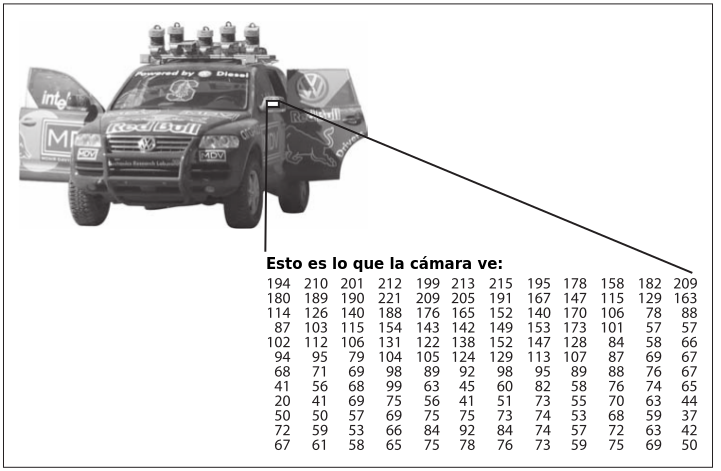
\includegraphics[width=0.5\textwidth]{Figures/representation_image.png}
    \end{figure}
\end{frame}

\begin{frame}\frametitle{Espacios de color}
  Son diferentes formas de representar el color.
  \begin{figure}
    \centering
    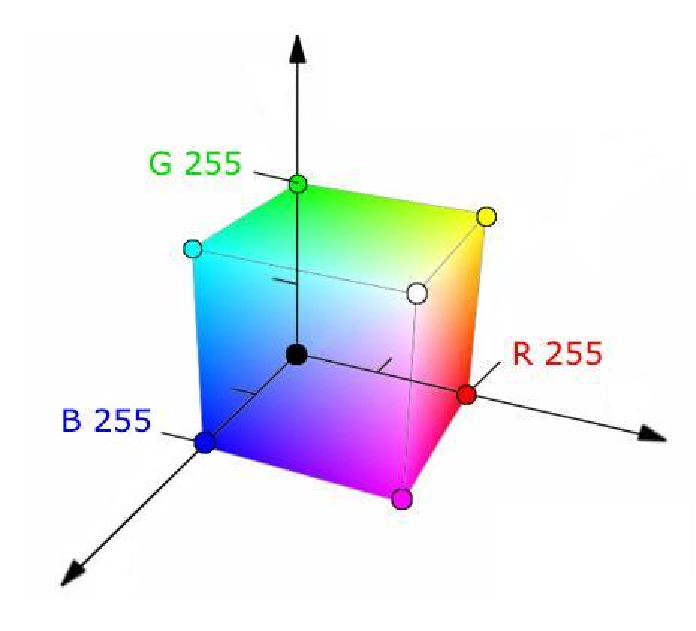
\includegraphics[width=0.35\textwidth]{Figures/RGB_model.pdf}
    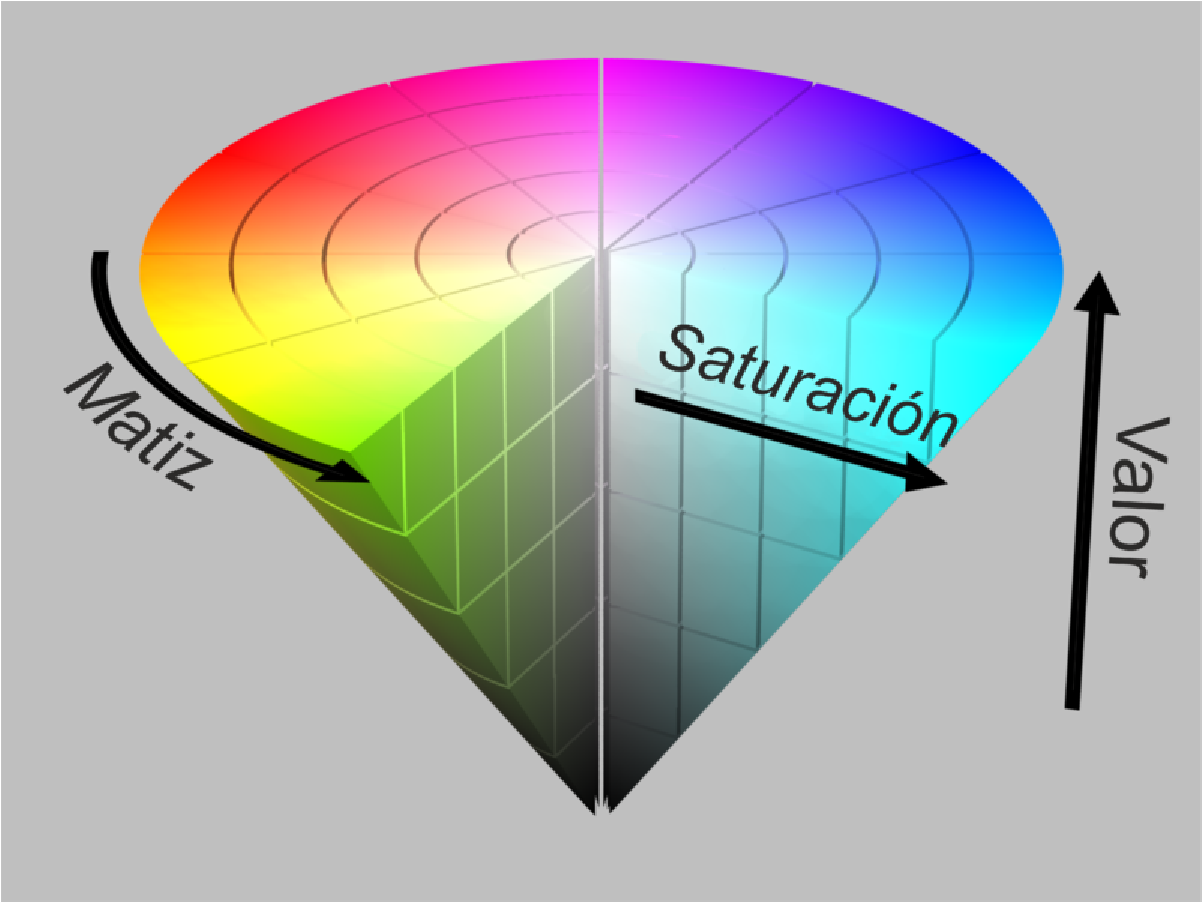
\includegraphics[width=0.35\textwidth]{Figures/hsv_space.pdf}
  \end{figure}
  En segmentación por color se recomienda más usar HSV, pues es más robusto ante cambios en la iluminación.
\end{frame}

\begin{frame}\frametitle{OpenCV y ROS}
  \begin{itemize}
  \item OpenCV utiliza la biblioteca Numpy para representar imágenes con matrices
  \item ROS representa las imágenes usando mensajes de tipo \texttt{sensor\_msgs/Image} o \texttt{sensor\_msgs/PointCloud2}.
  \item Para \textit{traducir} las imágenes entre los diferentes formatos, se utiliza el paquete \texttt{cv\_bridge} (\url{http://wiki.ros.org/cv_bridge}).
  \end{itemize}
\end{frame}

\begin{frame}\frametitle{Segmentación por color}
  La segmentación de una imagen se refiere a obtener regiones con ciertas características. En este caso, que estén en un cierto intervalo de color. Los pasos generales para esto son:
  \begin{enumerate}
  \item Transformación de la imagen del espacio BGR al HSV (función \texttt{cvtColor})
  \item Obtención de aquellos pixeles que están en un rango de color (función \texttt{inRange})
  \item Eliminación de \textit{outliers}, generalmente con operadores morfológicos (funciones \texttt{erode} y \texttt{dilate})
  \item Obtención de la posición de la región (funciones \texttt{findNonZero} y \texttt{mean})
  \end{enumerate}
\end{frame}

\begin{frame}\frametitle{Ejercicio}
  \begin{enumerate}
  \item Ejecutar el comando \texttt{roslaunch bring\_up robotino\_simul.launch}
  \item Ejecutar el nodo \texttt{rosrun vision color\_segmentation.py}
  \item Utilizando la ventana ``Image BGR'', obtener una captura de pantalla, guardarla y abrirla con cualquier editor de imágenes (Kolour Paint, por ejemplo) para obtener los valores HSV de la taza o de la lata de Cola-Cola.
    \item \textbf{Nota:} En OpenCV, los valores de \textit{Saturation} y \textit{Value} se almacenan como valores entre 0 y 255. El valor de \textit{Hue} es un ángulo y suele calcularse en grados, sin embargo, puesto que 360 no puede expresarse con 8 bits, OpenCV almacena la mitad del ángulo en el canal \textit{Hue}. 
  \item Modificar el archivo \texttt{catkin\_ws/src/vision/scripts/color\_segmentation.py}, en la función \texttt{inRange}, para segmentar correctamente la taza verde o la lata de Coca-Cola. Revisar la documentación en línea de dicha función (\url{https://docs.opencv.org/3.4/da/d97/tutorial_threshold_inRange.html}). 
  \end{enumerate}
\end{frame}

\begin{frame}\frametitle{La transformada SIFT}
  \begin{itemize}
  \item La transformada SIFT (Scale Invariant Feature Transform) es un algoritmo para obtener puntos característicos y sus descriptores sin que estos se vean afectados por la rotación o la escala.
  \item Esta transformada ya viene implementada en OpenCV (\url{https://docs.opencv.org/master/da/df5/tutorial_py_sift_intro.html})
  \item Es muy útil cuando los objetos a reconocer son ricos en texturas (bolsas de frituras, latas de refresco, etc)
  \item Si los objetos son lisos (platos, tazas, cubiertos), conviene más usar segmentación por color o forma.
  \end{itemize}
\end{frame}

\begin{frame}\frametitle{Reconocimiento de objetos con SIFT}
  El proceso general para entrenar, y posteriormente, reconocer un objeto, es el siguiente:

  \textbf{Entrenamiento:}
  \begin{enumerate}
  \item Tomar una foto del objeto aislado. Esta foto servirá como patrón.
  \item En OpenCv, crear un objeto de tipo \texttt{xfeatures2d.SIFT\_create} y mediante la función \texttt{detectAndCompute} obtener un conjunto de puntos característicos y sus descriptores.
  \item Almacenar dichos puntos y descriptores en un archivo. Puede ser binario, yaml, json, etc. En este curso se usará Json.
  \end{enumerate}

  \textbf{Reconocimiento:}
  \begin{enumerate}
  \item Cargar los puntos y descriptores del objeto que se desea reconocer. Estos serán los valores \textit{train}.
  \item En OpenCv, crear un objeto de tipo \texttt{xfeatures2d.SIFT\_create} y mediante la función \texttt{detectAndCompute} obtener un conjunto de puntos característicos y sus descriptores de la imagen de prueba. Estos serán los valores \textit{query}.
  \item Comparar los valores \textit{train} con los valores \textit{query} y obtener el subconjunto de valores \textit{query} que más se parece al conjunto \textit{train}. Si la diferencia es menor que un umbral, se puede considerar que el objeto entrenado está presente en la escena.
  \item Esta comparación se puede hacer con la función \texttt{knnMatch} de la clase \texttt{FlannBasedMatcher}.
  \end{enumerate}
\end{frame}

\begin{frame}\frametitle{Ejercicio}
  \begin{enumerate}
  \item Ejecutar el comando \texttt{roslaunch bring\_up robotino\_simul.launch}
  \item Ejecutar el nodo \texttt{rosrun vision sift\_detection.py}
  \item Tomar una captura de la ventana \texttt{Image BGR} y editarla para obtener una imagen como la de la figura, ya sea de la taza verde o la lata de Coca-Cola. El nombre del archivo no debe tener espacios.
    \begin{figure}
      \centering
      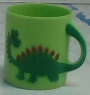
\includegraphics[width=0.15\textwidth]{Figures/GreenCup.png}
    \end{figure}
  \item Ejecutar el comando \texttt{rosrun vision sift\_training.py \_object\_name:=<NombreArchivo>}. El nombre del archivo es el de la imagen editada en el punto anterior sin extensión.
    \item Verificar que el archivo .json se haya generado correctamente. Este debería estar en la carpeta \texttt{catkin\_ws/src/vision/training}.
  \end{enumerate}
\end{frame}

\begin{frame}\frametitle{Ejercicio}
  \begin{enumerate}
  \item Ejecutar el nodo \texttt{rosrun vision sift\_recognition.py \_object\_name:=<NombreArchivo>}
  \item Verificar el correcto reconocimiento. Si no se logró, realizar uno de los siguientes ajustes:
    \begin{itemize}
    \item Modificar el umbral en la línea 37 de archivo \texttt{sift\_recognition.py},
      \item O la más recomendable: tomar otra captura y volver a entrenar. 
    \end{itemize}
  \end{enumerate}
\end{frame}

\begin{frame}\frametitle{Planeación de acciones}
  \begin{itemize}
  \item Máquinas de estados.
  \item Sistemas expertos, implementados con lenguajes lógicos como Prolog o CLIPS.
  \item Métodos probabilísticos, como MDPs.
  \end{itemize}
  Para las pruebas de @Home Beginners, las máquinas de estados son la mejor opción.
\end{frame}

\begin{frame}\frametitle{Planeación de acciones. Ejercicio}
Hacer programa para obedecer un comando de navegar a un lugar y buscar un objeto.
\end{frame}

\begin{frame}\frametitle{Contacto}
  Dr. Marco Negrete
  Profesor Asociado C
  Departamento de Procesamiento de Señales
  Facultad de Ingeniería, UNAM.

  mnegretev.info
  contact@mnegretev.info 
\end{frame}
\end{document}